\chapter{Fourier 变换}
\begin{figure}[h]
	\centering
	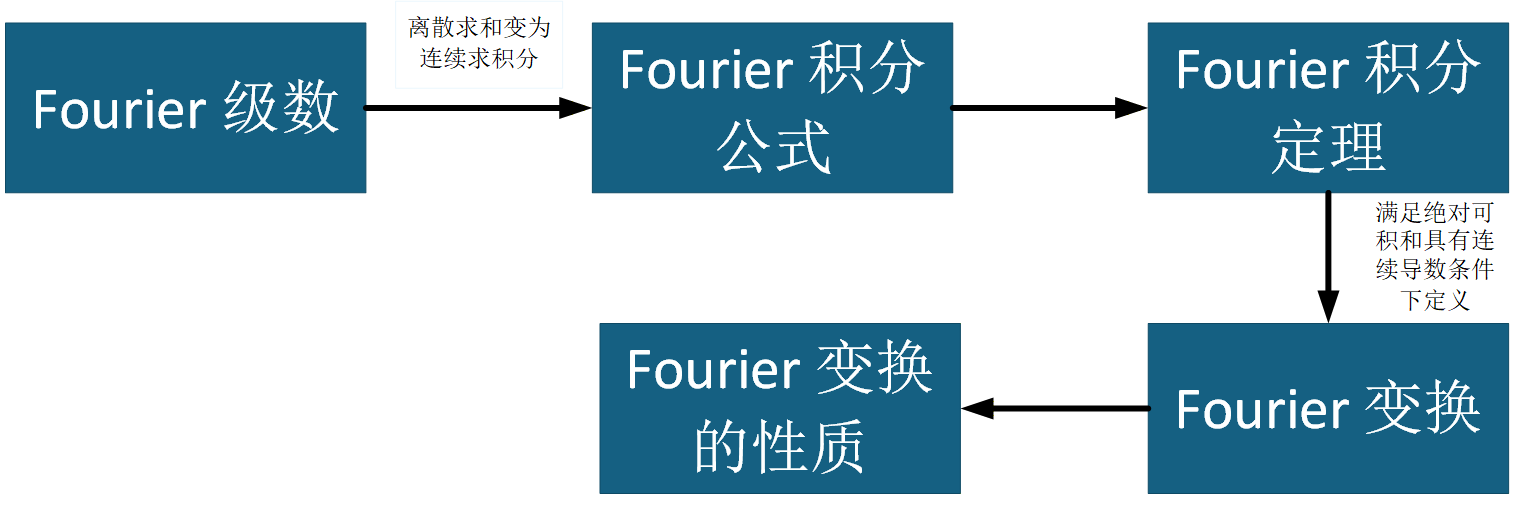
\includegraphics[width=0.7\linewidth]{Fourier变换}
	\caption{思维导图}
	
\end{figure}

\begin{theorem}[Fourier 级数定理]
	设周期为 $2l$ 的函数 $f(x)$ 在区间 $[-l,l]$ 上满足\textbf{狄利克雷条件}：
	\begin{enumerate}
		\item $f(x)$ 在 $[-l,l]$ 上分段连续；
		\item $f(x)$ 在 $[-l,l]$ 上只有有限个极值点。
	\end{enumerate}
	则 $f(x)$ 的 Fourier 级数
	\[
	\frac{a_0}{2}+\sum_{n=1}^{\infty}\left(a_n\cos\frac{n\pi x}{l}+b_n\sin\frac{n\pi x}{l}\right)
	\]
	在任意点 $x$ 处收敛，且其和为
	\[
	S(x)=
	\begin{cases}
		f(x), & x\text{ 为 }f(x)\text{ 的连续点},\\[4pt]
		\dfrac{f(x^-)+f(x^+)}{2}, & x\text{ 为 }f(x)\text{ 的间断点}.
	\end{cases}
	\]
	其中 Fourier 系数为
	\[
	\begin{aligned}
		a_n&=\dfrac{1}{l}\int_{-l}^{l}f(x)\cos\dfrac{n\pi x}{l}\,\mathrm{d}x,\quad n=0,1,2,\dots,\\
		b_n&=\dfrac{1}{l}\int_{-l}^{l}f(x)\sin\dfrac{n\pi x}{l}\,\mathrm{d}x,\quad n=1,2,\dots.
	\end{aligned}
	\]
	特别地，若周期为 $2\pi$（即 $l=\pi$），则系数简化为
	\[
	\begin{aligned}
		a_n&=\dfrac{1}{\pi}\int_{-\pi}^{\pi}f(x)\cos nx\,\mathrm{d}x,\quad n=0,1,2,\dots,\\
		b_n&=\dfrac{1}{\pi}\int_{-\pi}^{\pi}f(x)\sin nx\,\mathrm{d}x,\quad n=1,2,\dots.
	\end{aligned}
	\]
\end{theorem}

\begin{theorem}[Fourier 积分公式]
	若函数 $f(x)$ 在 $\mathbb R$ 上满足下列条件：
	\begin{enumerate}
		\item $f(x)$ 在任意有限区间上分段单调且分段连续；
		\item 广义积分 $\displaystyle\int_{-\infty}^{+\infty}|f(x)|\,\mathrm{d}x$ 收敛。
	\end{enumerate}
	则对任意 $x\in\mathbb R$，有
	\[
	\frac{f(x^-)+f(x^+)}{2}
	=\int_{0}^{+\infty}\left[A(\omega)\cos\omega x + B(\omega)\sin\omega x\right]\mathrm{d}\omega,
	\]
	其中
	\[
	A(\omega)=\frac{1}{\pi}\int_{-\infty}^{+\infty}f(t)\cos\omega t\,\mathrm{d}t,\quad
	B(\omega)=\frac{1}{\pi}\int_{-\infty}^{+\infty}f(t)\sin\omega t\,\mathrm{d}t.
	\]
	等价复指数形式为
	\[
	\frac{f(x^-)+f(x^+)}{2}
	=\frac{1}{2\pi}\int_{-\infty}^{+\infty}\left(\int_{-\infty}^{+\infty}f(t)e^{-i\omega t}\mathrm{d}t\right)
	e^{i\omega x}\mathrm{d}\omega.
	\]
	特别地，在 $f(x)$ 的连续点处有
	\[
	f(x)=\int_{0}^{+\infty}\big(A(\omega)\cos\omega x+B(\omega)\sin\omega x\big)\mathrm{d}\omega.
	\]
\end{theorem}

\begin{proof}
	由周期函数的 Fourier 级数展开，令周期 $2l\to+\infty$。
	设 $f(x)$ 满足定理条件，先将 $f(x)$ 在 $[-l,l]$ 上展开为 Fourier 级数：
	\[
	\frac{f(x^-)+f(x^+)}{2}
	=\frac{a_0}{2}+\sum_{n=1}^{\infty}\big(a_n\cos\omega_n x+b_n\sin\omega_n x\big),
	\]
	其中 $\omega_n=\dfrac{n\pi}{l}$，频率间隔 $\Delta\omega=\omega_{n+1}-\omega_n=\dfrac{\pi}{l}$，且
	\[
	a_n=\frac{1}{l}\int_{-l}^{l}f(t)\cos\omega_n t\,\mathrm{d}t,\quad
	b_n=\frac{1}{l}\int_{-l}^{l}f(t)\sin\omega_n t\,\mathrm{d}t.
	\]
	
	代入级数并整理：
	\[
	\frac{f(x^-)+f(x^+)}{2}
	=\frac{1}{2l}\int_{-l}^{l}f(t)\mathrm{d}t
	+\sum_{n=1}^{\infty}\frac{1}{l}\int_{-l}^{l}f(t)\cos\omega_n(x-t)\,\mathrm{d}t.
	\]
	
	令 $l\to+\infty$，由 $\displaystyle\int_{-\infty}^{+\infty}|f(t)|\mathrm{d}t$ 收敛，第一项趋于 $0$；
	再将离散求和过渡为连续积分 $\sum\limits_{n=1}^{\infty}\to\dfrac{l}{\pi}\displaystyle\int_{0}^{+\infty}\mathrm{d}\omega$，代入得
	\[
	\frac{f(x^-)+f(x^+)}{2}
	=\frac{1}{\pi}\int_{0}^{+\infty}\int_{-\infty}^{+\infty}f(t)\cos\omega(x-t)\,\mathrm{d}t\mathrm{d}\omega.
	\]
	展开余弦差角公式，即得实数形式 Fourier 积分公式。进一步利用 Euler 公式 $e^{\pm i\theta}=\cos\theta\pm i\sin\theta$，可等价推导出复指数形式，证毕。
\end{proof}


\begin{theorem}
	若 $\mathbb{R}$ 上的函数 $f(x)$ 满足下列条件：
	\begin{enumerate}
		\item $f(x)$ 在 $\mathbb{R}$ 上任一有限区间上满足 Dirichlet 条件；
		\item 积分 $\displaystyle\int_{-\infty}^{+\infty}|f(x)|\,\mathrm{d}x$ 收敛。
	\end{enumerate}
	则 $F(\lambda)=\displaystyle\int_{-\infty}^{+\infty}f(x)e^{-i\lambda x}\,\mathrm{d}x$ 在 $\mathbb{R}$ 上存在，且满足：
	\begin{enumerate}
		\item $\displaystyle\lim_{|\lambda|\to\infty}F(\lambda)=0$；
		\item $|F(\lambda)|\le\displaystyle\int_{-\infty}^{+\infty}|f(x)|\,\mathrm{d}x$；
		\item $F(\lambda)$ 在 $\mathbb{R}$ 上一致连续。
	\end{enumerate}
\end{theorem}

\begin{proof}
	(1) 由
	\[
	\int_{-\infty}^{+\infty}f(x)e^{-i\lambda x}\,\mathrm{d}x
	=\int_{-\infty}^{+\infty}f(x)\bigl(\cos\lambda x+i\sin(-\lambda x)\bigr)\,\mathrm{d}x,
	\]
	根据 Riemann-Lebesgue 引理，有
	\[
	F(\lambda)=\lim_{a\to+\infty}\int_{-a}^{a}f(x)\bigl(\cos\lambda x+i\sin(-\lambda x)\bigr)\,\mathrm{d}x,
	\]
	故 $\displaystyle\lim_{|\lambda|\to\infty}F(\lambda)=0$。
	
	(2)
	\[
	|F(\lambda)|
	=\left|\int_{-\infty}^{+\infty}f(x)e^{-i\lambda x}\,\mathrm{d}x\right|
	\le\int_{-\infty}^{+\infty}|f(x)|\left|e^{-i\lambda x}\right|\,\mathrm{d}x
	\le\int_{-\infty}^{+\infty}|f(x)|\,\mathrm{d}x.
	\]
	
	(3)
	\[
	|F(\lambda+h)-F(\lambda)|
	=\left|\int_{-\infty}^{+\infty}f(x)e^{-i(\lambda+h)x}\,\mathrm{d}x
	-\int_{-\infty}^{+\infty}f(x)e^{-i\lambda x}\,\mathrm{d}x\right|
	\]
	\[
	\le\int_{-\infty}^{+\infty}|f(x)|\cdot\left|e^{-ihx}-1\right|\,\mathrm{d}x = M,
	\]
	故 $F(\lambda)$ 在 $\mathbb{R}$ 上一致连续。
\end{proof}

\begin{theorem}[Fourier 积分定理]
	若 $\mathbb{R}$ 上的函数 $f(x)$ 绝对可积且具有连续导数 $f'(x)$，则对任意 $x\in\mathbb{R}$，有
	\[
	\frac{1}{2\pi}\,\mathrm{p.v.}\int_{-\infty}^{+\infty}F(\lambda)e^{i\lambda x}\,\mathrm{d}\lambda=f(x),
	\]
	其中 $F(\lambda)=\displaystyle\int_{-\infty}^{+\infty}f(x)e^{-i\lambda x}\,\mathrm{d}x$。
\end{theorem}

\begin{definition}
	若 $f(x)$ 满足 Fourier 积分定理条件，则称
	\[
	F(\lambda)=\int_{-\infty}^{+\infty}f(x)e^{-i\lambda x}\,\mathrm{d}x
	\]
	为 $f(x)$ 的 Fourier 变换，记为 $F(\lambda)=\mathcal{F}[f(x)]$ 或 $\hat{f}(\lambda)$。
	称
	\[
	f(x)=\frac{1}{2\pi}\int_{-\infty}^{+\infty}F(\lambda)e^{i\lambda x}\,\mathrm{d}\lambda
	\]
	为 $F(\lambda)$ 的 Fourier 逆变换，记为 $f(x)=\mathcal{F}^{-1}[F(\lambda)]$。
	并称 $F(\lambda)$ 与 $f(x)$ 为 Fourier 变换对，记为 $F(\lambda)\leftrightarrow f(x)$。
\end{definition}

\begin{definition}
	\begin{enumerate}
		\item 若 $f(x)$ 为奇函数，则
		\[
		F_s(\lambda)=\int_{0}^{+\infty}f(x)\sin\lambda x\,\mathrm{d}x
		\]
		称为 $f(x)$ 的 Fourier 正弦变换；
		\[
		f(x)=\frac{2}{\pi}\int_{0}^{+\infty}F_s(\lambda)\sin\lambda x\,\mathrm{d}\lambda
		\]
		称为 $F_s(\lambda)$ 的 Fourier 正弦逆变换。
		
		\item 若 $f(x)$ 为偶函数，则
		\[
		F_c(\lambda)=\int_{0}^{+\infty}f(x)\cos\lambda x\,\mathrm{d}x
		\]
		称为 $f(x)$ 的 Fourier 余弦变换；
		\[
		f(x)=\frac{2}{\pi}\int_{0}^{+\infty}F_c(\lambda)\cos\lambda x\,\mathrm{d}\lambda
		\]
		称为 $F_c(\lambda)$ 的 Fourier 余弦逆变换。
	\end{enumerate}
\end{definition}

\begin{definition}
	称满足
	\[
	\delta(t)=
	\begin{cases}
		0, & t\neq 0,\\
		\infty, & t=0,
	\end{cases}
	\quad
	\int_{-\infty}^{+\infty}\delta(t)\,\mathrm{d}t=1
	\]
	的函数为 Dirac 函数（单位脉冲函数）。其 Fourier 变换为
	\[
	\mathcal{F}[\delta(x)]=\int_{-\infty}^{+\infty}\delta(x)e^{-i\lambda x}\,\mathrm{d}x=1.
	\]
\end{definition}

\begin{theorem}
	Dirac 函数 $\delta(x)$ 具有如下性质：
	\begin{enumerate}
		\item 筛选性质：$\displaystyle\int_{-\infty}^{+\infty}\delta(x)\varphi(x)\,\mathrm{d}x=\varphi(0)$；
		\item 导数性质：$\displaystyle\int_{-\infty}^{+\infty}\delta^{(n)}(x)\varphi(x)\,\mathrm{d}x=(-1)^n\varphi^{(n)}(0)$；
		\item 对称性：$\delta(-x)=\delta(x)$；
		\item 伸缩性质：$\delta(ax)=\dfrac{1}{|a|}\delta(x)$；
		\item 乘积性质：$x\delta(x)=0$；
		\item 与阶跃函数关系：$\dfrac{\mathrm{d}}{\mathrm{d}x}H(x)=\delta(x)$，其中
		\[
		H(x)=
		\begin{cases}
			1, & x>0,\\
			0, & x<0
		\end{cases}
		\]
		为单位阶跃函数。
	\end{enumerate}
\end{theorem}
\begin{example}
	求单位阶跃函数 $H(x)$ 的 Fourier 变换。
\end{example}
\begin{proof}
	单位阶跃函数定义
	\[
	H(x)=
	\begin{cases}
		1, & x>0,\\
		0, & x<0.
	\end{cases}
	\]
	按 Fourier 变换定义
	\[
	\mathcal{F}[H(x)]
	=\int_{-\infty}^{+\infty}H(x)e^{-i\lambda x}\mathrm{d}x
	=\int_{0}^{+\infty}e^{-i\lambda x}\mathrm{d}x.
	\]
	取极限含主值积分与广义函数意义：
	\[
	\int_{0}^{+\infty}e^{-i\lambda x}\mathrm{d}x
	=\lim_{\varepsilon\to 0^+}\int_{0}^{+\infty}e^{-\varepsilon x}e^{-i\lambda x}\mathrm{d}x
	=\lim_{\varepsilon\to 0^+}\frac{1}{\varepsilon+i\lambda}.
	\]
	分解实部虚部并利用广义函数极限
	\[
	\lim_{\varepsilon\to 0^+}\frac{\varepsilon}{\lambda^2+\varepsilon^2}=\pi\delta(\lambda),\quad
	\lim_{\varepsilon\to 0^+}\frac{-\lambda}{\lambda^2+\varepsilon^2}=\frac{1}{i\lambda},
	\]
	因此
	\[
	\mathcal{F}[H(x)]=\frac{1}{i\lambda}+\pi\delta(\lambda).
	\]
\end{proof}

\begin{example}
	求 $f(x)=\sin\lambda_0 x$ 的 Fourier 变换。
\end{example}
\begin{solution}
	由欧拉公式
	\[
	\sin\lambda_0 x=\frac{e^{i\lambda_0 x}-e^{-i\lambda_0 x}}{2i}.
	\]
	已知基本变换公式
	\[
	\mathcal{F}\big[e^{i\lambda_0 x}\big]=2\pi\delta(\lambda-\lambda_0),\quad
	\mathcal{F}\big[e^{-i\lambda_0 x}\big]=2\pi\delta(\lambda+\lambda_0).
	\]
	线性性质得
	\[
	\begin{aligned}
		\mathcal{F}[\sin\lambda_0 x]
		&=\mathcal{F}\!\left[\frac{e^{i\lambda_0 x}-e^{-i\lambda_0 x}}{2i}\right]\\
		&=\frac{1}{2i}\Big[2\pi\delta(\lambda-\lambda_0)-2\pi\delta(\lambda+\lambda_0)\Big]\\
		&=i\pi\Big[\delta(\lambda+\lambda_0)-\delta(\lambda-\lambda_0)\Big].
	\end{aligned}
	\]
\end{solution}

\begin{example}
	求符号函数 $\operatorname{sgn}x$ 的 Fourier 变换。
\end{example}
\begin{solution}
	符号函数定义
	\[
	\operatorname{sgn}x=
	\begin{cases}
		1, & x>0,\\
		-1, & x<0.
	\end{cases}
	\]
	易知分解关系
	\[
	\operatorname{sgn}x = 2H(x)-1.
	\]
	由 Fourier 变换线性性
	\[
	\mathcal{F}[\operatorname{sgn}x]
	=2\mathcal{F}[H(x)]-\mathcal{F}[1].
	\]
	代入已知
	\[
	\mathcal{F}[H(x)]=\frac{1}{i\lambda}+\pi\delta(\lambda),\quad
	\mathcal{F}[1]=2\pi\delta(\lambda),
	\]
	则
	\[
	\begin{aligned}
		\mathcal{F}[\operatorname{sgn}x]
		&=2\left(\frac{1}{i\lambda}+\pi\delta(\lambda)\right)-2\pi\delta(\lambda)\\
		&=\frac{2}{i\lambda}+2\pi\delta(\lambda)-2\pi\delta(\lambda)\\
		&=\frac{2}{i\lambda}.
	\end{aligned}
	\]
\end{solution}

% ============================================================
% 一、线性性质
% ============================================================
\begin{theorem}[线性性质]
	若 $a,b$ 为常数，且 $\mathcal{F}[f(x)]=F(\lambda)$，$\mathcal{F}[g(x)]=G(\lambda)$，则
	\[
	\mathcal{F}[af(x)+bg(x)]=aF(\lambda)+bG(\lambda).
	\]
\end{theorem}

% ============================================================
% 二、位移性质（时移与频移）
% ============================================================
\begin{theorem}[位移性质]
	设 $\mathcal{F}[f(x)]=F(\lambda)$，则
	\begin{enumerate}
		\item 时移性质：
		\[
		\mathcal{F}[f(x\pm x_0)]=e^{\pm i\lambda x_0}F(\lambda).
		\]
		\item 频移性质：
		\[
		\mathcal{F}^{-1}[F(\lambda\pm\lambda_0)]=e^{\mp i\lambda_0 x}f(x).
		\]
	\end{enumerate}
\end{theorem}

\begin{proof}
	(1) 时移性质：
	\[
	\begin{aligned}
		\mathcal{F}[f(x+x_0)]
		&=\int_{-\infty}^{+\infty}f(x+x_0)e^{-i\lambda x}\,\mathrm{d}x \\
		&=e^{i\lambda x_0}\int_{-\infty}^{+\infty}f(x+x_0)e^{-i\lambda(x+x_0)}\,\mathrm{d}x \\
		&=e^{i\lambda x_0}\mathcal{F}[f(x)] = e^{i\lambda x_0}F(\lambda).
	\end{aligned}
	\]
	同理可证 $f(x-x_0)$ 的情况。
\end{proof}

\begin{example}
	设 $g(x)=e^{-\beta x}H(x)\cos\lambda_0 x\ (\beta>0)$，求 $\mathcal{F}[g(x)]$。
\end{example}
\begin{solution}
	设 $f(x)=\begin{cases}e^{-\beta x}, & x\ge 0,\\ 0, & x<0,\end{cases}$ 则 $g(x)=f(x)\cos\lambda_0 x$。
	由欧拉公式：
	\[
	\cos\lambda_0 x=\frac{e^{i\lambda_0 x}+e^{-i\lambda_0 x}}{2}.
	\]
	已知
	\[
	\mathcal{F}[f(x)]=\frac{1}{\beta+i\lambda}.
	\]
	由频移性质：
	\[
	\begin{aligned}
		\mathcal{F}[g(x)]
		&=\mathcal{F}\left[f(x)\cdot\frac{e^{i\lambda_0 x}+e^{-i\lambda_0 x}}{2}\right] \\
		&=\frac{1}{2}\mathcal{F}[f(x)e^{i\lambda_0 x}]+\frac{1}{2}\mathcal{F}[f(x)e^{-i\lambda_0 x}] \\
		&=\frac{1}{2}\cdot\frac{1}{\beta+i(\lambda-\lambda_0)}+\frac{1}{2}\cdot\frac{1}{\beta+i(\lambda+\lambda_0)}.
	\end{aligned}
	\]
\end{solution}

% ============================================================
% 三、微分性质
% ============================================================
\begin{theorem}[微分性质]
	设 $\lim\limits_{|x|\to\infty}f(x)=0$，且 $\mathcal{F}[f(x)]=F(\lambda)$，则
	\[
	\mathcal{F}[f'(x)]=i\lambda F(\lambda).
	\]
	更一般地，若 $\lim\limits_{|x|\to\infty}f^{(k)}(x)=0$，$k=0,1,\dots,n-1$，则
	\[
	\mathcal{F}[f^{(n)}(x)]=(i\lambda)^n F(\lambda).
	\]
	同时，若 $\lim\limits_{|\lambda|\to\infty}F(\lambda)=0$，则
	\[
	F^{(n)}(\lambda)=\mathcal{F}\left[(-i)^n x^n f(x)\right],
	\]
	即
	\[
	\mathcal{F}[x^n f(x)]=i^n F^{(n)}(\lambda).
	\]
\end{theorem}

\begin{proof}
	由分部积分法：
	\[
	\begin{aligned}
		\mathcal{F}[f'(x)]
		&=\int_{-\infty}^{+\infty}f'(x)e^{-i\lambda x}\,\mathrm{d}x \\
		&=\left.f(x)e^{-i\lambda x}\right|_{-\infty}^{+\infty} + i\lambda\int_{-\infty}^{+\infty}f(x)e^{-i\lambda x}\,\mathrm{d}x \\
		&= 0 + i\lambda F(\lambda) = i\lambda F(\lambda).
	\end{aligned}
	\]
\end{proof}

\begin{example}
	设 $f(x)=xe^{-\beta|x|}\ (\beta>0)$，求 $\mathcal{F}[f(x)]$。
\end{example}
\begin{solution}
	先求 $f_0(x)=e^{-\beta|x|}$ 的 Fourier 变换：
	\[
	\mathcal{F}[e^{-\beta|x|}]=\frac{2\beta}{\beta^2+\lambda^2}.
	\]
	由微分性质：
	\[
	\mathcal{F}[x f_0(x)] = i \frac{\mathrm{d}}{\mathrm{d}\lambda}\left(\frac{2\beta}{\beta^2+\lambda^2}\right)
	= i\cdot 2\beta \cdot \frac{-2\lambda}{(\beta^2+\lambda^2)^2}
	= i\left(\frac{2\beta}{\beta^2+\lambda^2}\right)'.
	\]
\end{solution}

% ============================================================
% 四、积分性质
% ============================================================
\begin{theorem}[积分性质]
	设 $g(x)=\int_{-\infty}^{x}f(t)\,\mathrm{d}t$，且 $\lim\limits_{x\to\infty}g(x)=0$，则
	\[
	\mathcal{F}[g(x)]=\frac{1}{i\lambda}\mathcal{F}[f(x)].
	\]
\end{theorem}

\begin{proof}
	由于 $g'(x)=f(x)$，且 $\lim\limits_{|x|\to\infty}g(x)=0$，由微分性质：
	\[
	\mathcal{F}[f(x)]=\mathcal{F}[g'(x)]=i\lambda\mathcal{F}[g(x)],
	\]
	故
	\[
	\mathcal{F}[g(x)]=\frac{1}{i\lambda}\mathcal{F}[f(x)].
	\]
\end{proof}

\begin{example}
	求解积分微分方程：
	\[
	x'(t)-\int_{-\infty}^{t}x(\tau)\,\mathrm{d}\tau=e^{-|t|}.
	\]
\end{example}
\begin{solution}
	设 $X(\lambda)=\mathcal{F}[x(t)]$。对方程两边做 Fourier 变换：
	\[
	\mathcal{F}[x'(t)]-\mathcal{F}\left[\int_{-\infty}^{t}x(\tau)\,\mathrm{d}\tau\right]=\mathcal{F}[e^{-|t|}].
	\]
	利用微分与积分性质：
	\[
	i\lambda X(\lambda)-\frac{1}{i\lambda}X(\lambda)=\frac{2}{\lambda^2+1}.
	\]
	整理得：
	\[
	X(\lambda)\left(i\lambda+\frac{i}{\lambda}\right)=\frac{2}{\lambda^2+1}
	\quad\Rightarrow\quad
	X(\lambda)\cdot\frac{i(\lambda^2+1)}{\lambda}=\frac{2}{\lambda^2+1}.
	\]
	解得：
	\[
	X(\lambda)=\frac{-2i\lambda}{(\lambda^2+1)^2}.
	\]
	做逆变换：
	\[
	x(t)=\mathcal{F}^{-1}\left[\frac{-2i\lambda}{(\lambda^2+1)^2}\right]=\frac{t}{2}e^{-|t|}.
	\]
\end{solution}

% ============================================================
% 五、相似性质（尺度变换）
% ============================================================
\begin{theorem}[相似性质]
	设 $\mathcal{F}[f(x)]=F(\lambda)$，常数 $a\neq 0$，则
	\[
	\mathcal{F}[f(ax)]=\frac{1}{|a|}F\left(\frac{\lambda}{a}\right).
	\]
	更一般地，
	\[
	\mathcal{F}[f(ax-x_0)]=\frac{1}{|a|}e^{-i\frac{\lambda x_0}{a}}F\left(\frac{\lambda}{a}\right).
	\]
\end{theorem}

\begin{proof}
	令 $u=ax$，则：
	\[
	\mathcal{F}[f(ax)]
	=\int_{-\infty}^{+\infty}f(ax)e^{-i\lambda x}\,\mathrm{d}x
	=\frac{1}{|a|}\int_{-\infty}^{+\infty}f(u)e^{-i\frac{\lambda}{a}u}\,\mathrm{d}u
	=\frac{1}{|a|}F\left(\frac{\lambda}{a}\right).
	\]
\end{proof}

% ============================================================
% 六、对称性质
% ============================================================
\begin{theorem}[对称性质]
	设 $\mathcal{F}[f(x)]=F(\lambda)$，则
	\[
	\mathcal{F}[F(x)]=2\pi f(-\lambda).
	\]
\end{theorem}

\begin{proof}
	由逆变换定义：
	\[
	f(x)=\frac{1}{2\pi}\int_{-\infty}^{+\infty}F(\lambda)e^{i\lambda x}\,\mathrm{d}\lambda.
	\]
	将 $x$ 与 $\lambda$ 互换，得：
	\[
	f(\lambda)=\frac{1}{2\pi}\int_{-\infty}^{+\infty}F(x)e^{i x\lambda}\,\mathrm{d}x.
	\]
	于是：
	\[
	\int_{-\infty}^{+\infty}F(x)e^{-i x\lambda}\,\mathrm{d}x
	=2\pi f(-\lambda),
	\]
	即 $\mathcal{F}[F(x)]=2\pi f(-\lambda)$。
\end{proof}

\begin{remark}
	若 $f(x)$ 为偶函数，则 $f(-x)=f(x)$，此时有
	\[
	\mathcal{F}[F(x)]=2\pi f(\lambda).
	\]
\end{remark}

% ============================================================
% 七、乘积定理与Parseval恒等式
% ============================================================
\begin{theorem}[乘积定理]
	设 $F_1(\lambda)=\mathcal{F}[f_1(x)]$，$F_2(\lambda)=\mathcal{F}[f_2(x)]$，则
	\[
	\int_{-\infty}^{+\infty}f_1(x)f_2(x)\,\mathrm{d}x
	=\frac{1}{2\pi}\int_{-\infty}^{+\infty}F_1(\lambda)\overline{F_2(\lambda)}\,\mathrm{d}\lambda.
	\]
	若 $f_1(x),f_2(x)$ 为实函数，则 $\overline{F_2(\lambda)}=F_2(-\lambda)$。
\end{theorem}

\begin{corollary}[Parseval 恒等式]
	设 $F(\lambda)=\mathcal{F}[f(x)]$，则
	\[
	\int_{-\infty}^{+\infty}|f(x)|^2\,\mathrm{d}x
	=\frac{1}{2\pi}\int_{-\infty}^{+\infty}|F(\lambda)|^2\,\mathrm{d}\lambda.
	\]
\end{corollary}

\begin{example}
	计算积分：
	\[
	\int_{-\infty}^{+\infty}\frac{\sin^2 x}{x^2}\,\mathrm{d}x.
	\]
\end{example}
\begin{solution}
	令 $f(x)=\dfrac{\sin x}{x}$，其 Fourier 变换为：
	\[
	F(\lambda)=\mathcal{F}\left[\frac{\sin x}{x}\right]
	=
	\begin{cases}
		\pi, & |\lambda|<1,\\
		0, & |\lambda|>1.
	\end{cases}
	\]
	由 Parseval 恒等式：
	\[
	\int_{-\infty}^{+\infty}\left(\frac{\sin x}{x}\right)^2\,\mathrm{d}x
	=\frac{1}{2\pi}\int_{-\infty}^{+\infty}|F(\lambda)|^2\,\mathrm{d}\lambda
	=\frac{1}{2\pi}\int_{-1}^{1}\pi^2\,\mathrm{d}\lambda
	=\frac{1}{2\pi}\cdot 2\pi^2 = \pi.
	\]
\end{solution}

% ============================================================
% 八、卷积定理
% ============================================================
\begin{definition}[卷积]
	设函数 $f_1(x),f_2(x)$，称积分
	\[
	(f_1*f_2)(x)=\int_{-\infty}^{+\infty}f_1(\tau)f_2(x-\tau)\,\mathrm{d}\tau
	\]
	为 $f_1(x)$ 与 $f_2(x)$ 的卷积。
\end{definition}

\begin{theorem}[卷积的性质]
	卷积满足：
	\begin{enumerate}
		\item 交换律：$f_1*f_2 = f_2*f_1$；
		\item 分配律：$f_1*(f_2+f_3)=f_1*f_2+f_1*f_3$；
		\item 结合律：$f_1*(f_2*f_3)=(f_1*f_2)*f_3$。
	\end{enumerate}
\end{theorem}

\begin{theorem}[卷积定理]
	设 $f_1(x),f_2(x)$ 满足 Fourier 积分定理条件，且
	\[
	\mathcal{F}[f_1(x)]=F_1(\lambda),\quad
	\mathcal{F}[f_2(x)]=F_2(\lambda),
	\]
	则
	\[
	\mathcal{F}[f_1(x)*f_2(x)]=F_1(\lambda)F_2(\lambda).
	\]
\end{theorem}